\PassOptionsToPackage{sorting=none}{biblatex}
\documentclass[
  bibliography=totoc,     % Literatur im Inhaltsverzeichnis
  captions=tableheading,  % Tabellenüberschriften
  titlepage=firstiscover, % Titelseite ist Deckblatt
]{scrartcl}

% Paket float verbessern
\usepackage{scrhack}

% Warnung, falls nochmal kompiliert werden muss
\usepackage[aux]{rerunfilecheck}

% unverzichtbare Mathe-Befehle
\usepackage{amsmath}
% viele Mathe-Symbole
\usepackage{amssymb}
% Erweiterungen für amsmath
\usepackage{mathtools}

% Fonteinstellungen
\usepackage{fontspec}
% Latin Modern Fonts werden automatisch geladen
% Alternativ zum Beispiel:
%\setromanfont{Libertinus Serif}
%\setsansfont{Libertinus Sans}
%\setmonofont{Libertinus Mono}

% Wenn man andere Schriftarten gesetzt hat,
% sollte man das Seiten-Layout neu berechnen lassen
\recalctypearea{}

% deutsche Spracheinstellungen
\usepackage[ngerman]{babel}


\usepackage[
  math-style=ISO,    % ┐
  bold-style=ISO,    % │
  sans-style=italic, % │ ISO-Standard folgen
  nabla=upright,     % │
  partial=upright,   % ┘
  warnings-off={           % ┐
    mathtools-colon,       % │ unnötige Warnungen ausschalten
    mathtools-overbracket, % │
  },                       % ┘
]{unicode-math}

% traditionelle Fonts für Mathematik
\setmathfont{Latin Modern Math}
% Alternativ zum Beispiel:
%\setmathfont{Libertinus Math}

\setmathfont{XITS Math}[range={scr, bfscr}]
\setmathfont{XITS Math}[range={cal, bfcal}, StylisticSet=1]

% Zahlen und Einheiten
\usepackage[
  locale=DE,                   % deutsche Einstellungen
  separate-uncertainty=true,   % immer Unsicherheit mit \pm
  per-mode=symbol-or-fraction, % / in inline math, fraction in display math
]{siunitx}

% chemische Formeln
\usepackage[
  version=4,
  math-greek=default, % ┐ mit unicode-math zusammenarbeiten
  text-greek=default, % ┘
]{mhchem}

% richtige Anführungszeichen
\usepackage[autostyle]{csquotes}

% schöne Brüche im Text
\usepackage{xfrac}

% Standardplatzierung für Floats einstellen
\usepackage{float}
\floatplacement{figure}{htbp}
\floatplacement{table}{htbp}

% Floats innerhalb einer Section halten
\usepackage[
  section, % Floats innerhalb der Section halten
  below,   % unterhalb der Section aber auf der selben Seite ist ok
]{placeins}

% Seite drehen für breite Tabellen: landscape Umgebung
\usepackage{pdflscape}

% Captions schöner machen.
\usepackage[
  labelfont=bf,        % Tabelle x: Abbildung y: ist jetzt fett
  font=small,          % Schrift etwas kleiner als Dokument
  width=0.9\textwidth, % maximale Breite einer Caption schmaler
]{caption}
% subfigure, subtable, subref
\usepackage{subcaption}

% Grafiken können eingebunden werden
\usepackage{graphicx}

% schöne Tabellen
\usepackage{booktabs}

% Verbesserungen am Schriftbild
\usepackage{microtype}

% Literaturverzeichnis
\usepackage[
  backend=biber,
]{biblatex}
% Quellendatenbank
\addbibresource{lit.bib}
\addbibresource{programme.bib}

% Hyperlinks im Dokument
\usepackage[
  german,
  unicode,        % Unicode in PDF-Attributen erlauben
  pdfusetitle,    % Titel, Autoren und Datum als PDF-Attribute
  pdfcreator={},  % ┐ PDF-Attribute säubern
  pdfproducer={}, % ┘
]{hyperref}
% erweiterte Bookmarks im PDF
\usepackage{bookmark}

% Trennung von Wörtern mit Strichen
\usepackage[shortcuts]{extdash}

\author{%
  Katharina Popp\\%
  \href{mailto:katharina.popp@tu-dortmund.de}{katharina.popp@tu-dortmund.de}%
  \and%
  Nicolai Weitkemper\\%
  \href{mailto:nicolai.weitkemper@tu-dortmund.de}{nicolai.weitkemper@tu-dortmund.de}%
}
\publishers{TU Dortmund – Fakultät Physik}


\subject{V601}
\title{Der Franck-Hertz-Versuch}
\date{
    Durchführung: 22.06.2021
    \hspace{3em}
    Abgabe: 29.06.2021
}

\begin{document}

\maketitle
\thispagestyle{empty}
\tableofcontents
\newpage

\section{Zielsetzung}

    Das Ziel dieses Versuches ist es,
    die Quantennatur von Elektronen zu untersuchen.\\
    Dazu werden die Energieverteilung der beschleunigten Elektronen
    sowie die Anregungsenergie von Quecksilber gemessen.

\section{Theorie} \label{sec:Theorie}

\subsection{Grundprinzip der elektrischen Brückenschaltungen}

   Elektrische Brückenschaltungen werden dazu verwendet, um unbekannte Größen, wie zum Bespiel Widerstände, Induktivitäten und
   Kapazitäten zu bestimmen.
   Dazu wird die Potentialdifferenz $U_\text{Br}$ zwischen zwei Punkten an der Schaltung gemessen.
   Mithilfe der Kirchhoff'schen Regeln lässt sich diese Brückenspannung $U_\text{Br}$ berechnen.
   \begin{enumerate}
       \item Die Knotenregel besagt, dass alle Ströme, die in einen Knoten hineinfließen, in der Summe gleich Null sein müssen.
       \begin{equation}
           \sum_k I_k = 0
       \end{equation}
       \item Die Maschenregel besagt, dass in einer Masche alle vorhandenen Spannungen in der Summe gleich Null sein müssen.
       \begin{equation}
           \sum_k U_k = 0
       \end{equation}
   \end{enumerate}

   % TODO: Grafik zur allgemeinen Brückenschaltung

   Daraus folgt für die Brückenspannung:

   \begin{equation}
       U_\text{Br} = \frac{R_2R_3 - R_1R_4}{(R_3 + R_4)(R_1 + R_2)} U_\text{S}
   \end{equation}
   Hierbei ist $U_\text{S}$ die Speisespannung des Stromkreises.
   Für das Verhältnis
   \begin{equation}
       R_1R_4 = R_2R_3 \label{eqn: Widerstände}
   \end{equation}
   verschwindet die Brückenspannung und man spricht von einer abgeglichenen Brücke.
   In den Brückenschaltungen sind Bauelemente enthalten, die als Abgleichelemente dienen.
   Dies sind Potentiometer, mit denen sich die ohmschen Widerstände in den Schaltungen variieren lassen, um
   die Brückenspannung auf Null zu regeln.
   Da die Speisespannung proportional zur Brückenspannung ist, sollte die Speisespannung möglichst hoch eingestellt werden,
   damit eine höhere Abgleichempfindlichkeit erzielt wird.
   Ziel ist es also, um eine unbekannte Größe zu bestimmen, die gegebenen Bauteile so einzustellen, dass
   die Brückenspannung gleich Null wird. Dann kann man aus den Beziehungen der bekannten Größen die Größen für das unbekannte Bauteil berechnen.

\subsection{Bestimmung der unbekannten Größen}

    \subsubsection{Messung von ohmschen Widerständen} \label{sec:Wheatstone}

        Um unbekannte Widerstände zu bestimmen, wird die Wheatstone'sche Brückenschaltung verwendet.
        Diese besteht nur aus ohmschen Widerständen und kann mit Gleich- und Wechselstrom betrieben werden.
        Der unbekannte Widerstand kann mithilfe der Gleichung \eqref{eqn: Widerstände} berechnet werden.
        Es gilt
        \begin{equation}
            R_x = R_2 \frac{R_3}{R_4} \; . \label{eqn: Rx}
        \end{equation}
        % TODO: EINER der Widerstände kann eingestellt werden. → Welcher?
        Die schon bekannten Widerstände $R_2$, $R_3$ und $R_4$ können durch ein Potentiometer so eingestellt werden,
        dass die Brückenspannung $U_\text{Br}$ gleich Null wird.
        Mit den so eingestellten Widerständen können die Größen für das unbekannte Bauteil berechnet werden.

    \subsubsection{Komplexe Widerstände}

        Bei der Verwendung von Kondensatoren mit einer Kapazität $C$ und Spulen mit einer Induktivität $L$ werden bei der Berechnung
        komplexe Widerstände verwendet. Als Speisespannung wird eine Wechselspannung eingesetzt.
        Komplexe Widerstände setzen sich aus einem Wirkwiderstand $X$ und einem Blindwiderstand $Y$ zusammen.
        Die allgemeine Darstellung lautet
        \begin{equation}
            \symbf{R} = X + jY \; .
        \end{equation}
        % TODO: …
        Für ohmsche Widerstände $R$, Kapazitäten $C$ und Induktivitäten $L$ werden durch
        \begin{align}
            %wird nicht wie gewünscht ausgegeben
            \symbf{R}_R = R, & \symbf{R}_C = - \frac{j}{\omega C}, & \symbf{R}_L = j \omega L
        \end{align}
        dargestellt.

    \subsubsection{Messung von Kapazitäten} \label{sec:Kapazität}

        Da bei einem realen Kondensator immer ein Teil der elektrischen Energie in Wärmeenergie umgewandelt
        wird und so verloren geht, wird mit dem Kondensator ein ohmscher Widerstand in Reihe geschaltet.
        Dieser ohmsche Widerstand wird mit Gleichung \eqref{eqn: Rx} berechnet.
        Für die Kapazität des Kondensators gilt
        \begin{equation}
            C_x = C_2 \frac{R_4}{R_3} \; . \label{eqn: Cx}
        \end{equation}
        Die Kapazität $C_2$ ist hierbei schon bekannt und ist mit einem Potentiometer, welches den bekannten Widerstand $R_2$ regelt,
        in Reihe geschaltet.

    \subsubsection{Messung von Induktivitäten} \label{sec:Induktivität}

        Auch bei einer realen Induktivität wird ein Teil der enthaltenen magnetischen Feldenergie in Wärmeenergie umgewandelt
        und geht verloren. Aus diesem Grund wird auch hier ein ohmscher Widerstand mit der Induktivität, zum Beispiel einer Spule,
        in Reihe geschaltet.
        Der ohmsche Widerstand kann wieder mit Gleichung \eqref{eqn: Rx} bestimmt werden.
        Die Induktivität wird durch
        \begin{equation}
            L_x = L_2 \frac{R_3}{R_4} \label{eqn: Lx}
        \end{equation}
        berechnet.
        Die Induktivität $L_2$ ist hier ebenfalls schon bekannt, und mit dem Potentiometer für $R_2$ in Reihe geschaltet.

    \subsubsection{Maxwell-Brücke} \label{sec:Maxwell}

        Eine weitere Möglichkeit, um Induktivitäten zu bestimmen, ist die Maxwell'sche Brückenschaltung.
        Die Elemente zum Abgleichen der Brücke sind hier $R_2$, $R_3$, $R_4$ und $C_4$, wobei $R_3$ und $R_4$ durch ein
        Potentiometer geregelt werden. Die Kapazität $C_4$ ersetzt die Induktivität $L_2$, da dies
        einfacher zu realisieren ist.
        Der Widerstand, der mit der Induktivität in Reihe geschaltet ist, lässt sich durch Gleichung \eqref{eqn: Rx} bestimmen,
        die Induktivität wird mit
        \begin{equation}
            L_x = R_2 R_3 C_4 \label{sec:LxMax}
        \end{equation}
        berechnet.

\subsection{Frequenzabhängige Brückenschaltungen}

    Alle komplexen Widerstände sind von der Frequenz $\omega$ der Speisespannung $U_\text{S}$ abhängig.
    Ist diese Frequenz zu hoch eingestellt, wird der Anteil der Streukapazitäten, die in den Bauteilen
    entstehen, zu groß, und ein Abgleichen ist nicht mehr möglich.
    Wenn die Frequenz zu niedrig ist, kommt es zu Problemen bei der technischen Handhabung,
    da nun einige Periodendauern für Einschwingvorgänge benötigt werden, bis sich eine stabile Brückenspannung $U_\text{Br}$
    eingestellt hat.
    Die Frequenzen sind optimal, wenn sich die Blind- und Wirkwiderstände einer Schaltung
    in einer Größenordnung befinden.

    \subsubsection{Die Wien-Robinson-Brücke} \label{sec:WR}

        In der Schaltung der Wien-Robinson-Brücke sind keine Abgleichelemente enthalten.
        Die Brückenspannung $U_\text{Br}$ soll in Abhängigkeit der Frequenz $\omega$ bestimmt werden.
        Es gilt:
        \begin{equation}
            \left\lvert \frac{U_\text{Br}}{U_\text{S}} \right\rvert = \frac{1}{9} \frac{(\Omega^2 - 1)^2}{(1 - \Omega^2)^2 + 9\Omega^2},
        \end{equation}
        %Betragsstriche an Größe des Quotienten anpassen.
        wobei
        \begin{equation}
            \Omega = \frac{\omega}{\omega_0} \label{eqn: GroßOmega}
        \end{equation}
        ist, mit
        \begin{equation}
            \omega_0 = \frac{1}{RC} \; . \label{eqn: omeganull}
        \end{equation}

        Die Wien-Robinson-Brücke filtert aus dem kontinuierlichen Frequenzspektrum die Frequenz $\omega_0$ heraus
        und schwächt die Frequenzen in der Nähe von $\omega_0$.
        Mit dieser Eigenschaft soll der Klirrfaktor gemessen werden, welcher dazu dient, die Qualität des
        Sinusgenerators zu prüfen.
        Wenn der Klirrfaktor hinreichend klein ist, ist auch der Anteil der Oberwellen, welche bei einem
        realen Sinusgenerator entstehen, gering.
        Der Generator wird auf die Frequenz $\omega_0$ geregelt, und übrig bleiben nur die von $\omega_0$
        verschiedenen Frequenzen.

    \subsubsection{Die TT-Brücke}

        Die TT-Brücke dient wie die Wien-Robinson-Brücke als elektronischer Filter.
        Der Unterschied liegt darin, dass die Spannungen $U_\text{S}$ und $U_\text{Br}$ gegen Masse
        angeschlossen werden können.
        Für das Spannungsverhältnis ergibt sich mit den Bezeichnungen
        aus den Gleichungen \eqref{eqn: GroßOmega} und \eqref{eqn: omeganull}:
        \begin{equation}
            \lvert \frac{U_\text{Br}}{U_\text{S}} \rvert = \frac{(\Omega^2 - 1)^2}{(1 - \Omega^2)^2 + 16\Omega^2}.
        \end{equation}

\clearpage

\section{Durchführung} \label{sec:Durchführung}
    Zu Beginn des Experiments werden die Reservoire aus \autoref{sec:Aufbau} mit einer abgemessenen Wassermenge (hier: $\SI{4}{\liter}$) befüllt.
    Anschließend werden im Abstand von $\symup{\Delta} t = \SI{1}{\minute}$ die Temperaturen $T_1$ und $T_2$, die Drücke $p_1$ und $p_2$, und die Leistungsaufnahme des Kompressors $N$ gemessen.
    Auf den abgelesenen Wert des Drucks muss zusätzlich ein Wert von $\SI{1}{\bar}$ addiert werden.
    Bei einer Temperatur von $\SI{50}{\celsius}$ soll die Messung abgebrochen werden.

\clearpage

\section{Auswertung} \label{sec:Auswertung}
Die zur Verfügung gestellten Messdaten sind im Folgenden tabellarisch aufgelistet:
\begin{table}[H]
\centering
\caption{Aufgenommene Messdaten}
\label{tab:Messdaten}
\sisetup{table-format=2.1}
\begin{tabular}{c c c c c c}
\toprule
$t \mathbin{/} \si{\minute}$ &
$T_1 \mathbin{/} \si{\celsius}$ &
$p_1 \mathbin{/} \si{\bar}$ &
$T_2 \mathbin{/} \si{\celsius}$ &
$p_2 \mathbin{/} \si{\bar}$ &
$N \mathbin{/} \si{\watt}$ \\
\midrule
%  Messdaten zur Wärmepumpe
%  4l Wasser, Wärmekapazität der ´Kupferschlangen`: mkck = 750 J/K
%
%  t[min] T1 [C] p1[bar] T2[C] p2 [bar] N [W]
0	 & 21.7 & 4.0  & 21.7 & 4.1 & 120 \\
1  & 23.0 & 5.0  & 21.7 & 3.2	& 120 \\
2  & 24.3 & 5.5  & 21.6 & 3.4	& 120 \\
3  & 25.3 & 6.0  & 21.5 & 3.5	& 120 \\
4  & 26.4 & 6.0  & 20.8 & 3.5	& 120 \\
5  & 27.5 & 6.0  & 20.1 & 3.4	& 120 \\
6  & 28.8 & 6.5  & 19.2 & 3.3	& 120 \\
7  & 29.7 & 6.5  & 18.5 & 3.2	& 120 \\
8  & 30.9 & 7.0  & 17.7 & 3.2	& 120 \\
9  & 31.9 & 7.0  & 16.9 & 3.0	& 120 \\
10 & 32.9 & 7.0  & 16.2 & 3.0	& 120 \\
11 & 33.9 & 7.5  & 15.5 & 2.9	& 120 \\
12 & 34.8 & 7.5  & 14.9 & 2.8	& 120 \\
13 & 35.7 & 8.0  & 14.2 & 2.8	& 120 \\
14 & 36.7 & 8.0  & 13.6 & 2.7	& 120 \\
15 & 37.6 & 8.0  & 13.0 & 2.6	& 120 \\
16 & 38.4 & 8.5  & 12.4 & 2.6	& 120 \\
17 & 39.2 & 8.5  & 11.7 & 2.6	& 120 \\
18 & 40.0 & 9.0  & 11.3 & 2.5	& 120 \\
19 & 40.7 & 9.0  & 10.9 & 2.5	& 120 \\
20 & 41.4 & 9.0  & 10.4 & 2.4	& 120 \\
21 & 42.2 & 9.0  & 9.9  & 2.4	& 120 \\
22 & 42.9 & 9.5  & 9.5  & 2.4	& 120 \\
23 & 43.6 & 9.5  & 9.1  & 2.4	& 120 \\
24 & 44.3 & 0.0	 & 8.7  & 2.4	& 120 \\
25 & 44.9 & 0.0	 & 8.3  & 2.4	& 120 \\
26 & 45.5 & 0.0	 & 8.0  & 2.3	& 120 \\
27 & 46.1 & 0.0	 & 7.7  & 2.2	& 122 \\
28 & 46.7 & 0.5	 & 7.4  & 2.2	& 122 \\
29 & 47.3 & 0.5	 & 7.1  & 2.2	& 122 \\
30 & 47.8 & 0.75 & 6.8  & 2.2	& 122 \\
31 & 48.4 & 1.0	 & 5.6  & 2.2	& 122 \\
32 & 48.9 & 1.0	 & 4.3  & 2.2	& 122 \\
33 & 49.4 & 1.0	 & 3.4  & 2.2	& 122 \\
34 & 49.9 & 1.0	 & 3.0  & 2.2	& 122 \\
35 & 50.3 & 1.0	 & 2.9  & 2.2	& 122 \\
\bottomrule
\end{tabular}
\end{table}


\newpage
\subsection{Diagramm der gemessenen Temperaturverläufe} % a)
In \autoref{fig:plot} sind die Approximationen aus \autoref{eqn:approx_poly} in \autoref{sec:approx} bereits enthalten.
Dargestellt sind die zeitlichen Verläufe der Temperaturen $T_1$ und $T_2$ [TODO …der Reservoire].

\begin{figure}
  \centering
  \includegraphics{build/wärmepumpe_plot.pdf}
  \caption{Temperaturverläufe in Abhängigkeit der Zeit $t$.}
  \label{fig:plot}
\end{figure}

\subsection{Approximation der Temperaturverläufe} \label{sec:approx} % b)
Zur Approximation des Temperaturverläufe bietet sich ein Polynom zweiten Grades an:
\begin{equation}
  \label{eqn:approx_poly}
  T(t) = At^2 + Bt + C \; .
\end{equation}

Als Fit-Parameter wurden berechnet:

\begin{table}
\centering
\caption{Fit-Parameter}
\label{tab:fit_params}
% \sisetup{table-format=2.1}
\begin{tabular}{c c c c}
\toprule
 & A & B & C \\
\midrule
% $T_1$ &
% \num{-3.2249e-06} ± \num{4.1934e-08} &
% \num{0.02028} ± \num{9.1105e-05} &
% \num{294.97} ± \num{0.041345}\\
% $T_2$ &
% \num{9.5504e-07} ± \num{2.6711e-07} &
% \num{-0.011209} ± \num{0.00058032} &
% \num{295.87} ± \num{0.26336}\\
\input{../build/table_polyfit.tex}
\bottomrule
\end{tabular}
\end{table}

\subsection{Berechnung von Differentialquotienten} % c)
Mithilfe der Approximation aus Gleichung \autoref{eqn:approx_poly} werden nun für vier verschiedene Temperaturen konkrete Differentialquotienten $\frac{\mathrm{d}T_1}{\mathrm{d}t}$ und $\frac{\mathrm{d}T_2}{\mathrm{d}t}$ berechnet.
Die Ableitung des Polynoms lautet:
\[
\frac{\mathrm{d}T}{\mathrm{d}t} = 2At + B \; .
\]
\\

Fehlerrechnung:
\begin{align*}
  \symup{\Delta} \frac{\mathrm{d}T}{\mathrm{d}t}
  &= \sqrt{\left(\frac{\partial \frac{\mathrm{d}T}{\mathrm{d}t}}{\partial A} \cdot \symup{\Delta} A\right)^2 + \left(\frac{\partial \frac{\mathrm{d}T}{\mathrm{d}t}}{\partial B} \cdot \symup{\Delta} B\right)^2} \\
  &= \sqrt{(2t \cdot \symup{\Delta} A)^2 + (\symup{\Delta} B)^2} \; .
\end{align*}

\begin{table}
\centering
\caption{Ableitungen der Approximationsfunktion}
\label{tab:derivatives}
\sisetup{table-format=2.1}
\begin{tabular}{c c c c c c}
\toprule
$t \,/\, \si{\minute}$ &
$\frac{\mathrm{d}T_1}{\mathrm{d}t} \,/\, \si{\celsius\per\minute}$ &
$\frac{\mathrm{d}T_2}{\mathrm{d}t} \,/\, \si{\celsius\per\minute}$ \\
\midrule
7  & \num{0.017571}  ± \num{0.000098}  & \num{-0.010406}  ± \num{0.000622} \\
14 & \num{0.014862}  ± \num{0.000115}  & \num{-0.0096042} ± \num{0.0007336} \\
21 & \num{0.012153}  ± \num{0.000140}  & \num{-0.0088020} ± \num{0.0008887} \\
28 & \num{0.0094441} ± \num{0.0001678} & \num{-0.0079998} ± \num{0.0010688} \\

% 7  & \num{1.757e-02} ± \num{0.010e-02} & \num{-1.041e-02} ± \num{0.062e-02} \\
% 14 & \num{1.486e-02} ± \num{0.012e-02} & \num{-9.604e-03} ± \num{0.734e-03} \\
% 21 & \num{1.215e-02} ± \num{0.014e-02} & \num{-8.802e-03} ± \num{0.889e-03} \\
% 28 & \num{9.444e-03} ± \num{0.168e-03} & \num{-8.000e-03} ± \num{1.069e-03} \\


\bottomrule
\end{tabular}
\end{table}


\subsection{Bestimmung der Güteziffern} % d)
\label{sec:auswertung_gueteziffern}
% In "Daten und Hinweise" ist lediglich die Rede vom *Fassungsvermögen*!
% „Fassungsvermögen der Wassereimer: m = 4kg“
% Als Füllmenge nehmen wir daher 4L an, wie es in "Daten.dat" steht

% „Wärmekapazität der Kupferschlangen“ meint *Wärmekapazität jeder Kupferschlange*, oder?
Jeder Wassereimer war mit $\SI{4}{\liter}$ Wasser befüllt, bei einem Fassungsvermögen von $\SI{4}{\kilo\gram}$.
Die Wärmekapazität der \enquote{Kupferschlangen} war gegeben als $m_k c_k = \SI{750}{\joule\per\kelvin}$. Laut Versuchsanleitung soll $m_k c_k$ auch die Wärmekapazität der Eimer enthalten, dazu liegen jedoch keine weiteren Daten vor.
Die Wärmekapazität des Wassers in Reservoir 1 lässt sich mit
\begin{align*}
  \rho_\text{Wasser} &= \SI{0.998207}{\kilo\gram\per\liter}
  \tag*{(Wasserdichte bei 20°C \cite{wasserdichte})} \\
  \\
  c_\text{Wasser} &= \SI{4.1851}{\joule\per\gram\and\kelvin}
  \tag*{(spezifische Wärmekapazität von Wasser bei 20°C \cite{wasserwaermekapazitaet})} \\
  \\
  C_{\text{Wasser}, 1} &= m_1 \cdot c_\text{Wasser} \\
  &= (\rho_\text{Wasser} \cdot V_\text{Wasser}) \cdot c_\text{Wasser} \\
  &= \left(\SI{0.998207}{\kilo\gram\per\liter} \cdot \SI{4}{\liter}\right) \cdot \SI{4.181}{\joule\per\gram\and\kelvin} \\
  &= \SI{16736.0}{\joule\per\kelvin} \\
\end{align*}
bestimmen, sodass aus einfacher Summation die gesamte Wärmekapazität
\[
C_\text{ges} = 750 \si{\joule\per\kelvin} + \SI{16736.0}{\joule\per\kelvin} = \SI{17486.0}{\joule\per\kelvin}
\]
folgt.

\ \\
Unter Zuhilfenahme von Gleichung \ref{eqn:reale_gueteziffer} und der Differentialquotienten aus Tabelle \ref{tab:derivatives} kann nun die reale Güteziffer für verschiedene $t$ berechnet werden.

\begin{table}
\centering
\caption{Vergleich der idealen und realen Güteziffern}
% \sisetup{table-format=2.1}
\begin{tabular}{c c c c c c}
\toprule
$t \,/\, \si{\minute}$ &
$\nu_\text{ideal}$ &
$\nu_\text{real}$ \\
% TODO: Abweichung in % dazu?
\midrule
7  & 27.04 ± 0.34  & 2.560 ± 0.014 \\
14 & 13.41 ± 0.08  & 2.166 ± 0.017 \\
21 & 9.76  ± 0.04  & 1.771 ± 0.020 \\
28 & 8.139 ± 0.028 & 1.354 ± 0.024 \\
\bottomrule
\end{tabular}
\end{table}

\subsection{Bestimmung des Massendurchsatzes} % e)
% e) Man errechne für die 4 Temperaturen aus 5c den Massendurchsatz des hier benutzten Transportgases Dichlordifluormethan (Cl 2 F 2 C). Die Verdampfungswärme L dieses Stoffes kann man aus seiner Dampfdruck-Kurve gewinnen. (Näheres hierzu findet man in V203.) Wertepaare (p,T) zur Darstellung dieser Kurve können an den Manometern der Apparatur abgelesen werden. Mit den dort abgelesenen (p, T)-Werten führe man eine Ausgleichsrechnung zur Bestimmung von L durch.

% TODO: Verschieben zur Theorie → 1.1.2

! Dieser Abschnitt ist \textbf{work-in-progress} !

universelle Gaskonstante $R$

\begin{align*}
  \frac{1}{p} \mathrm{d}p &= \frac{L}{R \cdot T^2} \mathrm{d} T \\
  \mathrm{ln}(p) &= \frac{L}{R} \cdot \frac{1}{T} + c \\
  \mathrm{ln}(p) &= \frac{L}{R \cdot T} + c \\
  \mathrm{ln}(p) \cdot (R \cdot T) &= L + c \\
\end{align*}

\begin{table}
\centering
\caption{Massendurchsatz}
% \sisetup{table-format=2.1}
\begin{tabular}{c c c c c c}
\toprule
$t \,/\, \si{\second}$ &
$\frac{\mathrm{d}T_2}{\mathrm{d}t} \,/\, \SI{e-3}{\kelvin\per\second}$ &
$\frac{\mathrm{d}m}{\mathrm{d}t} \,/\, \si{\gram\per\second}$ \\
% TODO: Abweichung in % dazu?
\midrule
% 7  | deriv: (-1.041+/-0.062)e-02 & -1.54+/-0.09 TODO \\
% 14 | deriv: (-9.604+/-0.734)e-03 & -1.42+/-0.11 TODO \\
% 21 | deriv: (-8.802+/-0.889)e-03 & -1.30+/-0.13 TODO \\
% 28 | deriv: (-8.000+/-1.069)e-03 & -1.18+/-0.16 TODO \\
\input{../build/table_massendurchsatz.tex}
\bottomrule
\end{tabular}
\end{table}


\subsection{Bestimmung der Kompressorleistung} % f)
Die mechanische Leistung des Kompressors, die dieser abgibt, wenn
er zwischen den Drücken $p_1$ und $p_2$ arbeitet,
wird mithilfe von Gleichung \ref{eqn:N_mech}, der gegebenen Daten, und der Differentialquotienten aus Tabelle \ref{tab:derivatives} berechnet.
\ \\
Daten für $\mathrm{Cl}_2 \mathrm{F}_2 \mathrm{C}$: \\
% \[
$ρ_0 = \SI{5.51} g/l$ bei $T = \SI{0}{\celsius}$ und $p = \SI{1}{\bar}$, $κ = 1.14$
% \]

\begin{table}
\centering
\caption{Kompressorleistung}
% \sisetup{table-format=2.1}
\begin{tabular}{c c c c c c}
\toprule
% $t \,/\, \si{\second}$ &
% $\frac{\mathrm{d}T_2}{\mathrm{d}t} \,/\, \SI{e-3}{\kelvin\per\second}$ &
% $\frac{\mathrm{d}m}{\mathrm{d}t} \,/\, \si{\gram\per\second}$ \\

$t \,/\, \si{\second}$ &
% $\rho \,/\, \si{\kilo\gram\per\meter³}$ &
$ N_\text{mech} \,/\, \si{\watt}$ \\
\midrule
\input{../build/table_kompressorleistung.tex}
\bottomrule
\end{tabular}
\end{table}

\clearpage

\section{Diskussion} \label{sec:diskussion}

\subsection{Abweichungen}

Die relative Abweichung der Messwerte wird als
\begin{equation*}
  \symup{\Delta}\chi = \frac{\chi_{R/U} - \chi_T}{\chi_T}
\end{equation*}
angegeben.
Daraus ergeben sich die Abweichungen,
die in \autoref{tab:abweichungen} aufgelistet sind.

\begin{table}
  \centering
  \caption{Abweichung der experimentell bestimmten Suszeptibilitäten von den Theoriewerten.}
  \label{tab:abweichungen}
  \begin{tabular}{c S S}
  \toprule
  Stoff &
  {$\symup{\Delta} \chi_R$ [\%]} &
  {$\symup{\Delta} \chi_U$ [\%]} \\
  \midrule
  $\symup{Dy_2O_3}$ & -11.94 & -67.25 \\
  $\symup{Nd_2O_3}$ & - 2.38 &  90.16 \\
  \bottomrule
  \end{tabular}
\end{table}

Die Abweichungen entsprechen in etwa dem,
was mit Blick auf die Messwerte zu erwarten war.
Die Spannungsdifferenzen $\symup{\Delta}U$ fielen beispielsweise in allen drei Messungen mit $\symup{Nd_2O_3}$ sehr unterschiedlich aus
und waren sehr klein gegenüber ihrem Fehler.
Entsprechend groß ist die Abweichung mit $\num{90.16}\%$.


\subsection{Mögliche Fehlerquellen}

Beim Einstellen des Abgleichwiderstands zeigte sich,
dass das verwendete Spannungsmessgerät nicht hinreichend genau abgelesen werden konnte:
Für einen gewissen Einstellbereich war auf dem Messgerät keine Änderung zu erkennen.
Es ist daher mit einer Abweichung des Widerstands von circa $\pm\SI{50}{\milli\ohm}$ zu rechnen.
Das entspricht rund $\num{50}\%$ der in \autoref{tab:messwerte_U_R} gelisteten $\symup{\Delta}R$ und kann zu entsprechend großen Fehlern führen.
% Spannung ging nicht auf 0 runter… ¯\_(ツ)_/¯


Der bestimmte reale Querschnitt $Q_\text{real}$ unterliegt einem systematischen Fehler,
da die Röhrchen nicht vollständig gefüllt waren,
aber die Länge des gesamten Teströhrchens gemessen wurde.
Daraus resultieren zu niedrige Werte.
% - Röhrchen nicht ganz gefüllt, nicht ganz in der Spule…


Die \hyperref[fig:plot_filterkurve]{Filterkurve} fiel mit einer \hyperref[misc:güte]{Güte von $8.7611 \pm 0.0164$} breit aus.
Dadurch konnten Störfrequenzen die gemessene Spannung stärker verfälschen.


Die Suszeptibilität der Proben ist bekanntlich auch von deren Temperatur abhängig.
Zwar wurde versucht, die Proben nicht durch längeren Hautkontakt zu erwärmen,
allerdings variierte möglicherweise auch die Umgebungstemperatur nicht unerheblich,
da ein nahegelegenes Fenster geöffnet war.


% - diverse Probleme im Vorhinein…
% - 100mV_eff

\clearpage

\printbibliography
\clearpage

\appendix
\section{Messwerte}

\begin{figure}
    \centering
    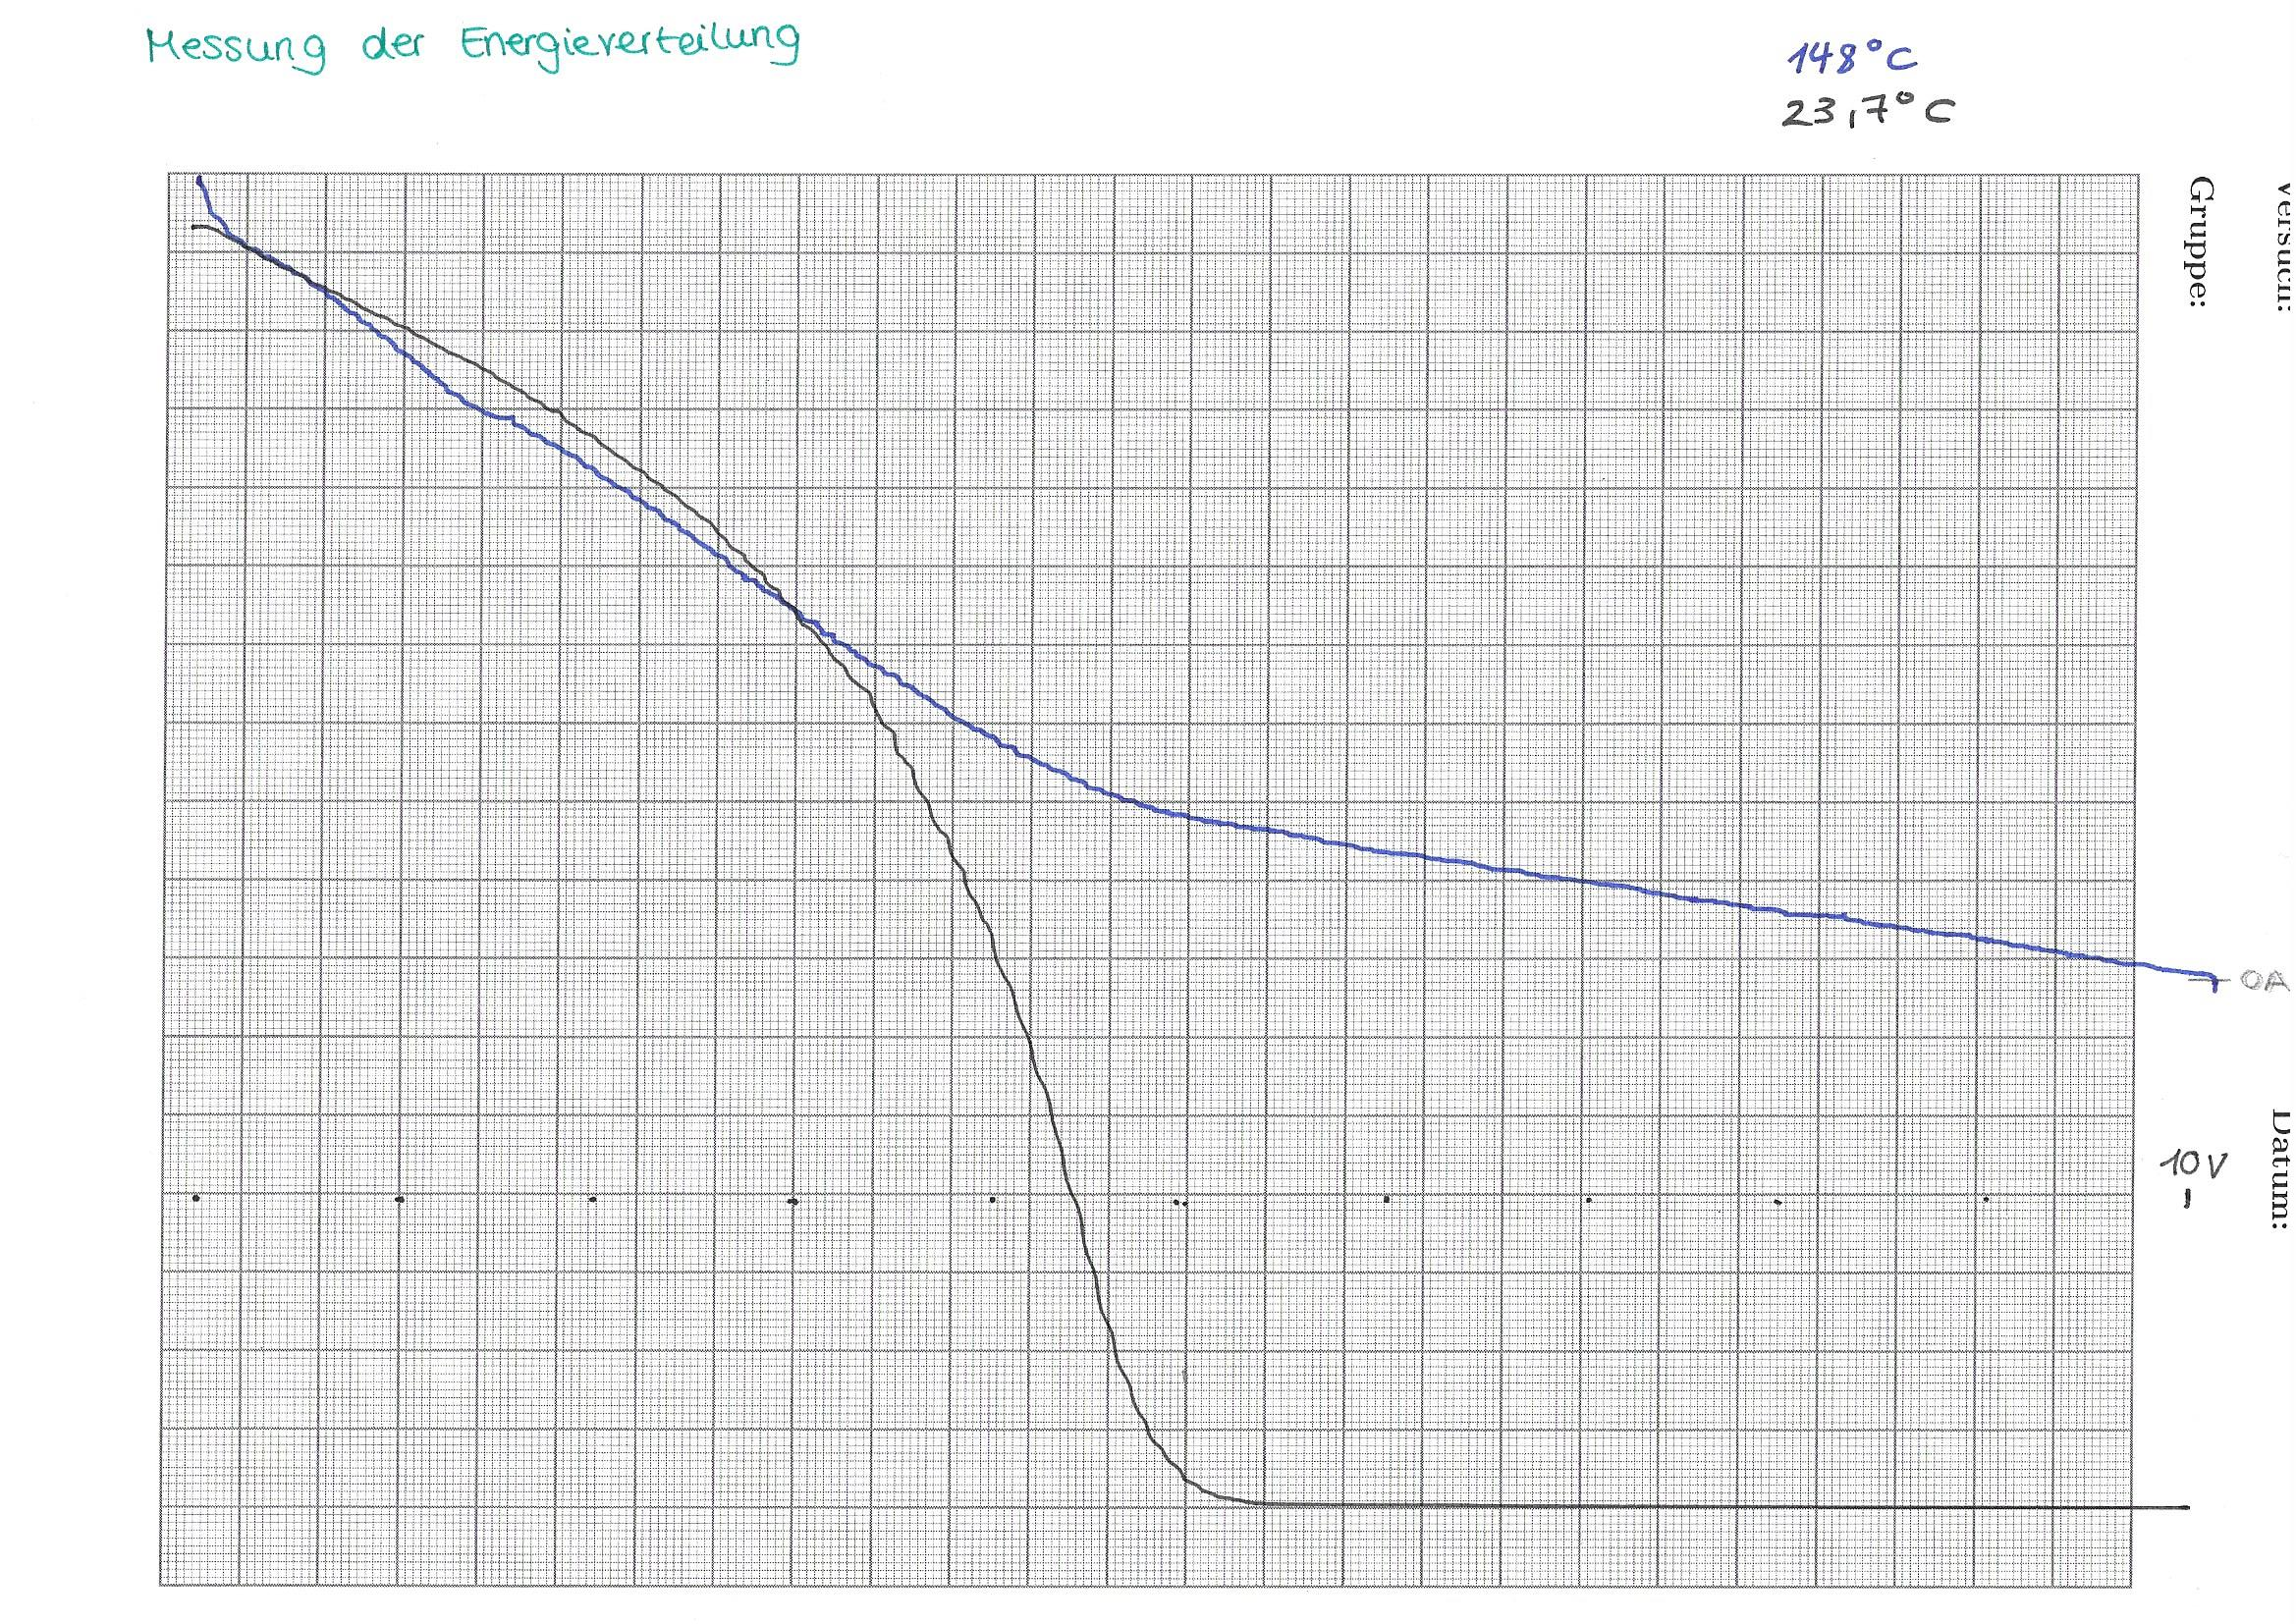
\includegraphics[width=\textwidth]{content/img/mess_energieverteilung.jpg}
    \caption{Mit dem XY-Schreiber aufgenommene Graphen zur Energieverteilung der Elektronen.}
    \label{fig:mess_energieverteilung}
\end{figure}

\begin{figure}
    \centering
    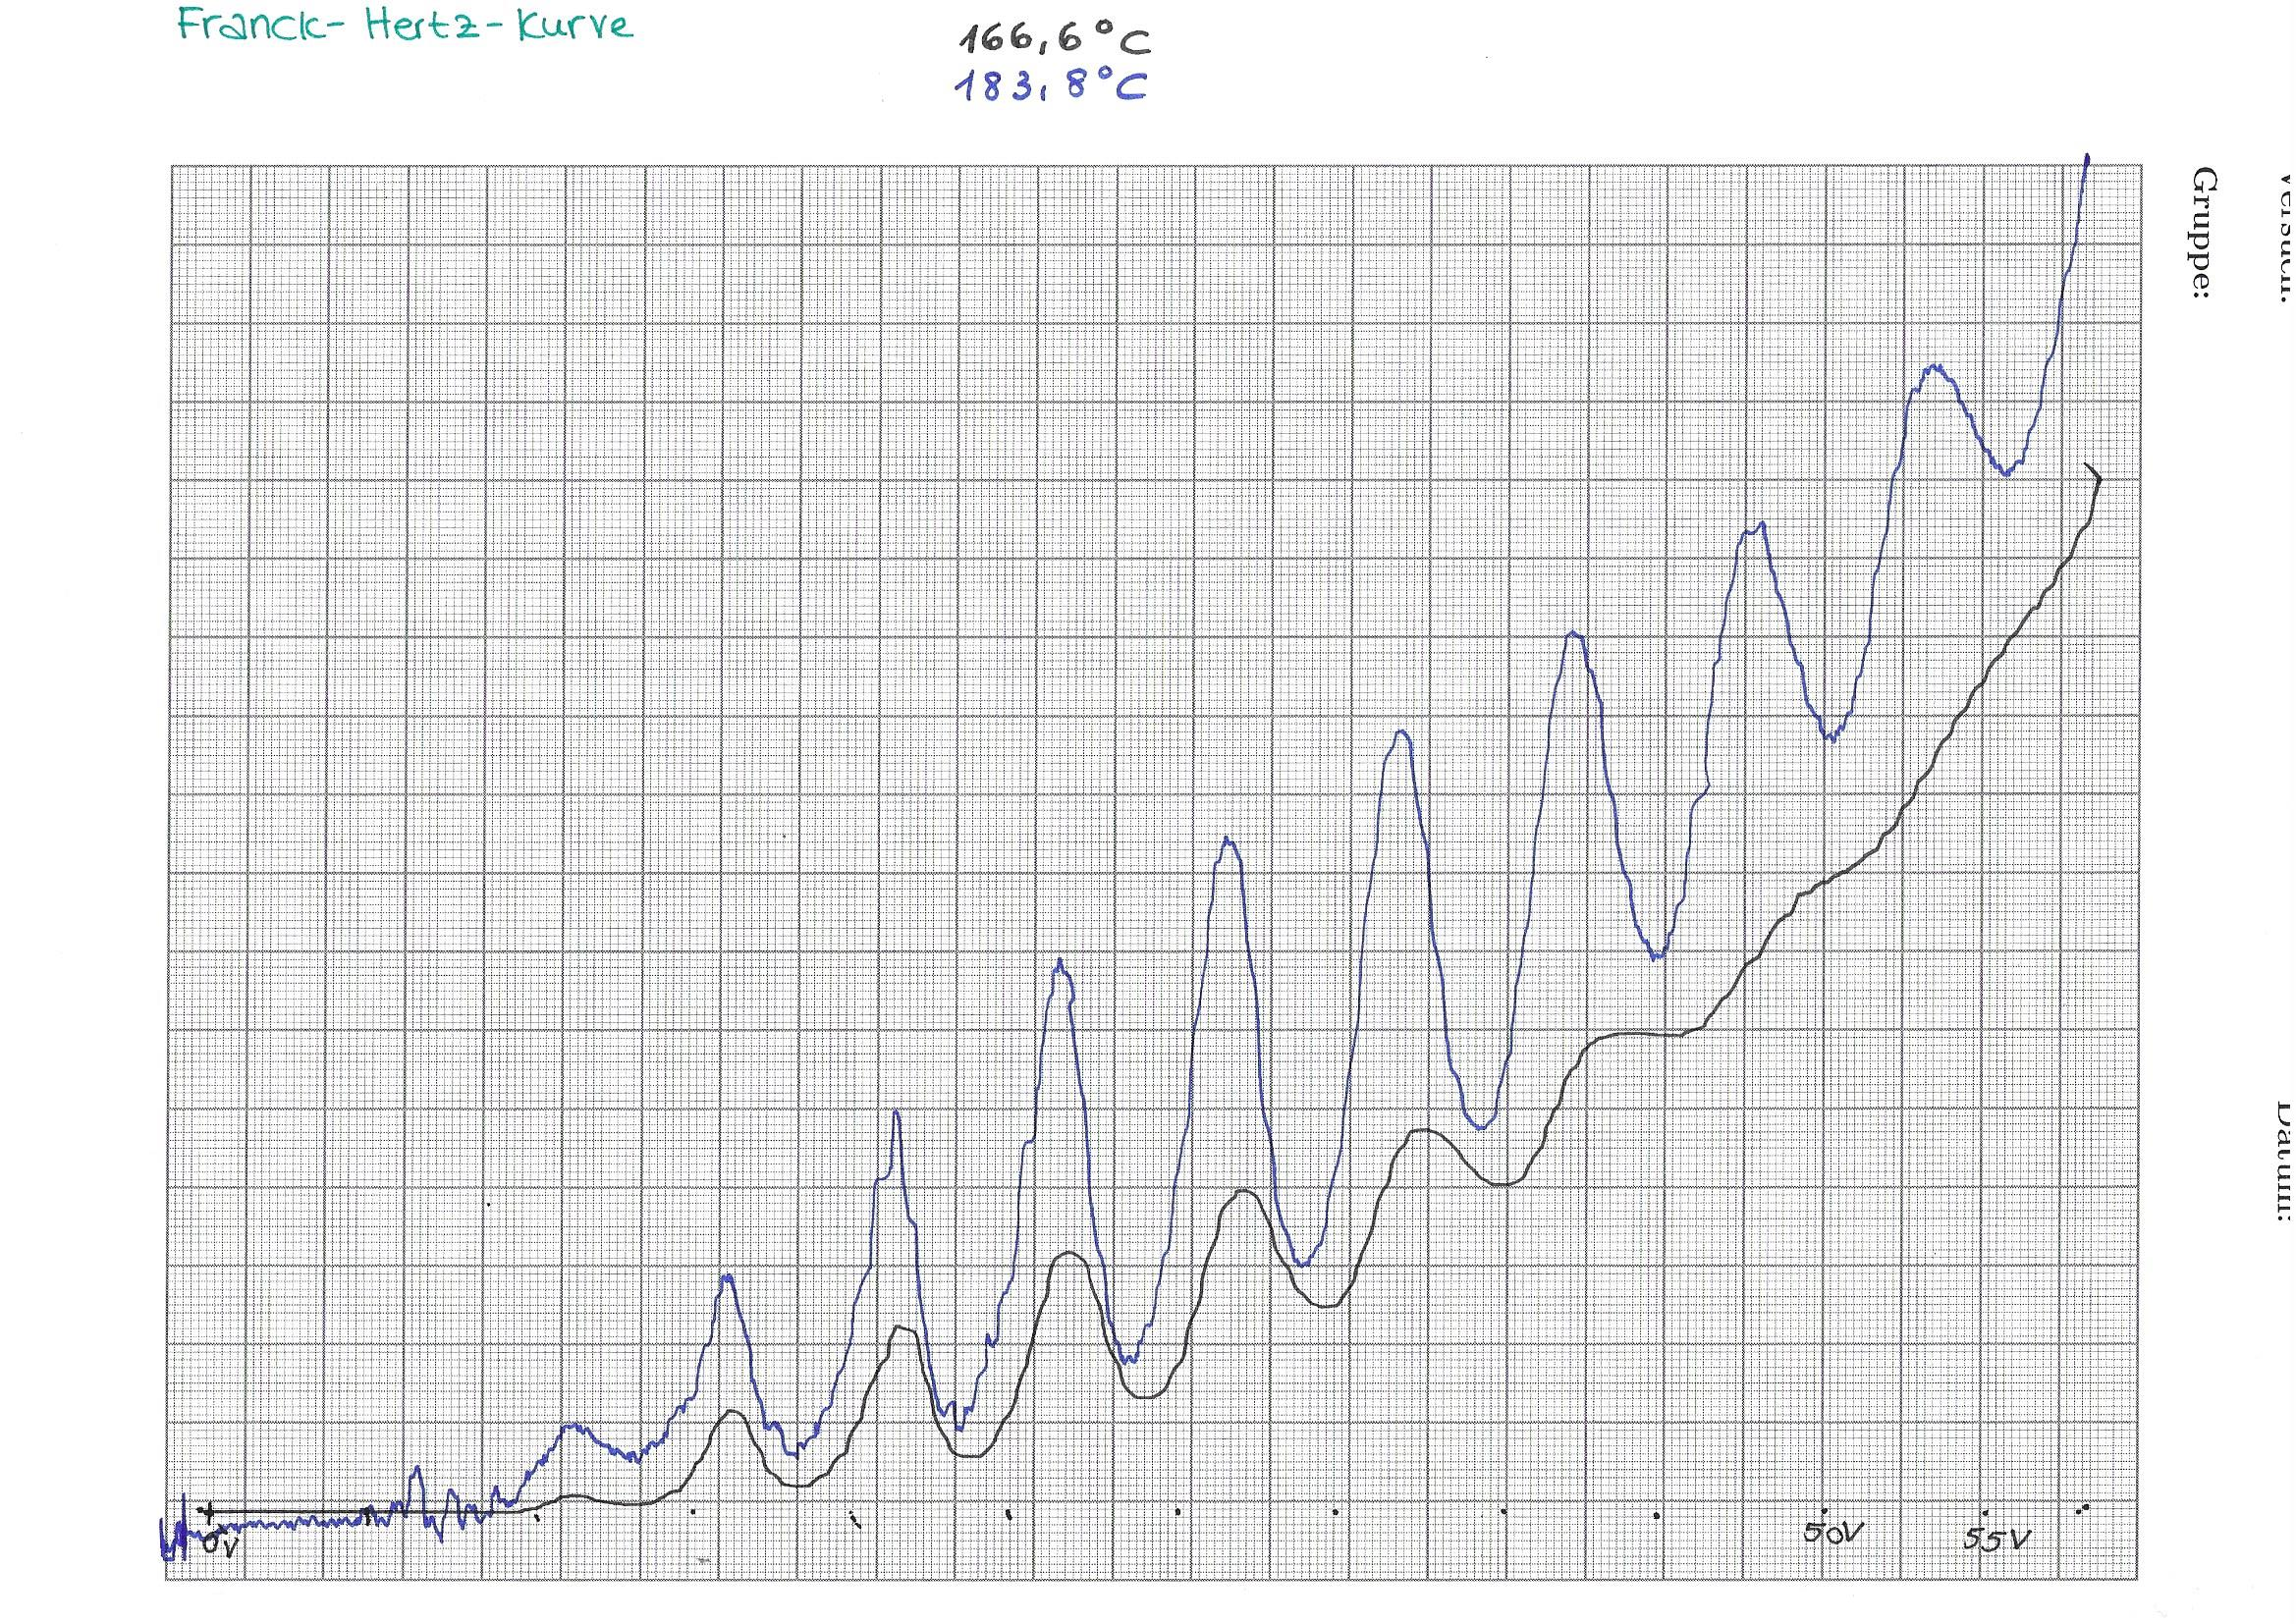
\includegraphics[width=\textwidth]{content/img/mess_franck_hertz.jpg}
    \caption{Mit dem XY-Schreiber aufgenommene Franck-Hertz-Kurven.}
    \label{fig:mess_franck_hertz}
\end{figure}


\end{document}
